%% LyX 2.0.5 created this file.  For more info, see http://www.lyx.org/.
%% Do not edit unless you really know what you are doing.
\documentclass{article}
\usepackage{amsmath}
\usepackage{amssymb}
\usepackage{fontspec}
\setmonofont{Times New Roman}
\usepackage{geometry}
\geometry{verbose,tmargin=1.5cm,bmargin=1.5cm,lmargin=1cm,rmargin=1cm}
\usepackage{wasysym}
\usepackage{graphicx}

\makeatletter

%%%%%%%%%%%%%%%%%%%%%%%%%%%%%% LyX specific LaTeX commands.
\newcommand{\noun}[1]{\textsc{#1}}
%% Because html converters don't know tabularnewline
\providecommand{\tabularnewline}{\\}
%% A simple dot to overcome graphicx limitations
\newcommand{\lyxdot}{.}


%%%%%%%%%%%%%%%%%%%%%%%%%%%%%% Textclass specific LaTeX commands.
\newenvironment{lyxcode}
{\par\begin{list}{}{
\setlength{\rightmargin}{\leftmargin}
\setlength{\listparindent}{0pt}% needed for AMS classes
\raggedright
\setlength{\itemsep}{0pt}
\setlength{\parsep}{0pt}
\normalfont\ttfamily}%
 \item[]}
{\end{list}}
\newenvironment{lyxlist}[1]
{\begin{list}{}
{\settowidth{\labelwidth}{#1}
 \setlength{\leftmargin}{\labelwidth}
 \addtolength{\leftmargin}{\labelsep}
 \renewcommand{\makelabel}[1]{##1\hfil}}}
{\end{list}}

\makeatother

\begin{document}
\begin{lyxcode}
\input{\string"Aussagelogik und Elementare Mengenlehre/Aussagelogik_und_Elementare_Mengenlehre.tex\string"}


\part*{Funktionen}


\section*{Funktionen (Grundlagen)}


\subsection*{Trigonometrische Funktionen}
\begin{quote}
\begin{tabular}{cc}
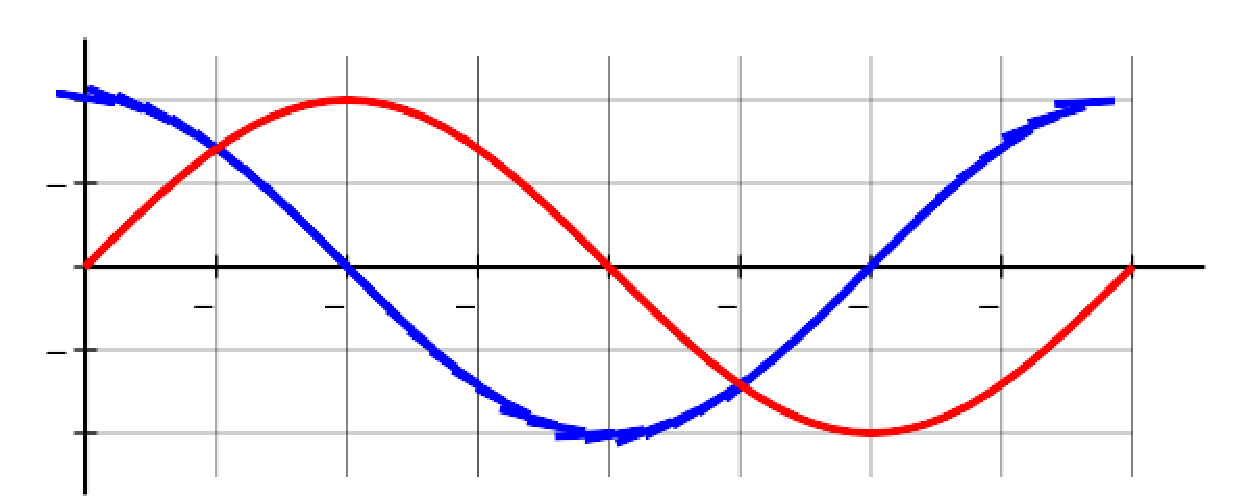
\includegraphics[width=6cm]{Funktionen/Sine_cosine_one_period} & 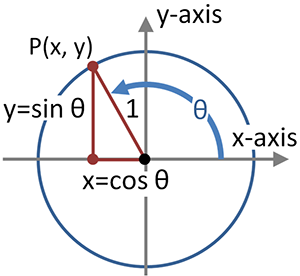
\includegraphics[width=5cm]{Funktionen/trigfun}\tabularnewline
\end{tabular}
\end{quote}

\subsection*{Polynome}
\begin{quote}
Ein Polynom n-ter Ordnung: $p(x)=a_{n}x^{n}+...+a_{2}x^{2}+a_{1}x+a_{0,}x\in R,a_{n}\neq0$
\end{quote}
Eigenschaften:
\begin{itemize}
\item Differenzen und Summen von Polynomen sind wieder Polynome.
\item Produkte von Polynomen sind wieder Polynome. Bsp: $p(2)\times p(3)=p(5)$
\item Die Division von Polynomen ergiebt wieder ein Polynom und ev. einen
Rest.
\end{itemize}
Beispiel für Polynomdivision:
\begin{verse}
\begin{tabular}{cccccc}
$2x$$^{3}$ & $+5x$$^{2}$ & $+1x$ & $\div(x-5)$ & $=$ & $2x^{2}-5x$ Rest $-24x$\tabularnewline
\hline 
$-2x^{3}$ & $-10x^{2}$ &  & $2x^{2}\times(x-5)$ & $=$ & $2x^{3}-10x^{2}$\tabularnewline
\cline{1-2} 
$0$ & $-5x^{2}$ & $+1x$ & $-5x\times(x-5)$ & $=$ & $-5x^{2}+25x$\tabularnewline
\cline{2-3} 
 & $-(-5x^{2})$ & $-25x$ &  &  & \tabularnewline
\cline{2-3} 
 & $0$ & $-24x$ &  &  & Rest: $-24x$\tabularnewline
\end{tabular}
\end{verse}

\subsubsection*{Hornerschema}

Auswertung einer Funktion an einer bestimmten Stelle.
\begin{verse}
Sei die Funktion $F(x)=x^{3}-3x^{2}-10x+24=(x-2)(x^{2}-x-12)$
\end{verse}
Diese an $x=2$ ausgewertet:
\begin{verse}
\begin{tabular}{ccccc}
\hline 
\multicolumn{1}{|c}{x=2} & $x^{3}$ & $-3x^{2}$ & $-10x$ & \multicolumn{1}{c|}{$24$}\tabularnewline
\hline 
 & 1 & -3 & -10 & 24\tabularnewline
 &  & 2 & -2 & -24\tabularnewline
\hline 
 & 1 & -1 & -12 & 0\tabularnewline
\hline 
Rest: & $x^{2}$ & $-x$ & $-12$ & \tabularnewline
\end{tabular}
\end{verse}
Hier wurde die Nullstelle $x=2$ abgespalten.


\subsection*{Begriffe der Funktionen}


\subsubsection*{Ganz-Rationale Funktion}

Eine Ganz-Rationale Funktion lässt sich so schreiben: $f(x)=a_{n}x^{n}+...+a_{2}x^{2}+a_{1}x+a_{0}$


\subsubsection*{Gebrochen-Rationale Funktion}

Eine Gebrochen-Rationale Funktion: $f(x)=\frac{a_{n}x^{n}+...+a_{2}x^{2}+a_{1}x+a_{0}}{b_{n}x^{n}+...+b_{2}x^{2}+b_{1}x+b_{0}}=\frac{p(m)}{p(n)}$,
wobei der Grad der Polynome nicht gleich sein muss.


\subsubsection*{Definitionslücken}

Sie sind Stellen, an denen die Funktion nicht definiert ist. Z.B.:
Nenner der gleich 0 ist. Man unterscheidet 2 Arten von Definitionslücken:
\begin{itemize}
\item Polstellen: Nach dem vollständigen Kürzen, besteht immernoch die Nullstelle
des Nenners.
\item hebbare Definitionslücken: Nach vollständigem Kürzen verschwindet
die Nullstelle des Nenners.
\item Stopfen der Def. Lücke: Wert der hebbaren Lücke in den gekürzten Bruch
einsetzen. 
\end{itemize}
Wichtig: Kommt eine Polstelle mehrmals vor: $(x-a)^{n}$, so ist dies
eine n-fache Polstelle. Ist die Vielfachheit gerade, so findet kein
Vorzeichenwechsel statt.


\subsubsection*{Nullstellen}

Man kann die Nullstellen bestimmen, indem man:
\begin{itemize}
\item bei einer ``Ganz-Rationalen Funktion'' diese gleich NULL setzt.
\item bei einer ``Gebrochen-Rationalen Funktion'' den Zähler gleich NULL
setzt.
\end{itemize}

\subsubsection*{Asymptoten}

Sind Geraden, denen sich eine Kurve beliebig nahe annähert. Wir unterscheiden
2 Arten:
\begin{itemize}
\item bei Polstellen: Die Kurve einer gebrochen-rationalen Funktion schmiegt
sich der Gerade bei x=Polstelle an. Es bildet sich eine senkrechte
Asymptote.
\item für grosse x: $f(x)=\frac{g(x)}{h(x)}$ im Falle:

\begin{itemize}
\item $grad(g)<grad(h)$: x-Achse als wagrechte Asymptote
\item $grad(g)=grad(h)$: Gerade mit der Gleichung: $f(x)=\frac{g(x)}{h(x)}$
\item $grad(g)=1+grad(h)$: schiefe Asymptote, durch Polynomdivision
\end{itemize}
\end{itemize}
Man beachte beim Zeichnen die Vielfachheit der Polstelle:
\begin{itemize}
\item Gerade Anzahl: Vorzeichenwechsel
\item Ungerade Anzahl: Kein Vorzeichenwechsel
\end{itemize}
\begin{tabular}{|c|c|}
\hline 
Gerade & Ungerade\tabularnewline
\hline 
$\frac{x^{2}-1}{(x+1)^{2}}$ & $\frac{x^{2}-1}{(x+1)^{3}}$\tabularnewline
\hline 
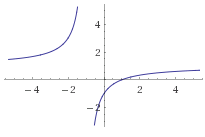
\includegraphics{Funktionen/vrzw} & 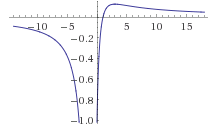
\includegraphics{Funktionen/kvrzw}\tabularnewline
\hline 
\end{tabular}


\subsubsection*{Beispiele:}
\begin{verse}
\begin{tabular}{|c|c|c|}
\hline 
Funktion & Definitionslücke & Nullstelle\tabularnewline
\hline 
\hline 
$f(x)=\frac{(x+2)^{2}}{(x+4)^{3}x^{2}}$ & P:-4(x3), 0(x2), H: keine & N:-2(x2)\tabularnewline
\hline 
\end{tabular}
\end{verse}


Betrachten wir die Funktion: $f(x)=\frac{2x^{2}+x^{2}+x}{1-x^{2}}$

Nullstelle: $x=0$

Definitionslücken: $x=$1 (Polstelle, 1fach), $x=-1$ (Polstelle,
1fach)

Asymptoten: $x=1$, $x=-1$, $x=-2x-1$ (durch Poly.division)


\subsection*{Umkehrfunktionen}


\subsubsection*{Begriffe}
\begin{verse}
\begin{tabular}{|c|c|c|}
\hline 
injektive Funktion & surjektive Funktion & bijektive funktion\tabularnewline
\hline 
\hline 
\includegraphics[width=2.5cm]{Funktionen/Injection\lyxdot svg} & \includegraphics[width=2.5cm]{Funktionen/Surjection\lyxdot svg} & \includegraphics[width=2.5cm]{Funktionen/Bijection\lyxdot svg}\tabularnewline
\hline 
\end{tabular}
\end{verse}

\subsubsection*{Monotonie}

Die Funktion $f(x)$ ist im Intervall $[a,b]$ injektiv, falls sie:
\begin{itemize}
\item streng monoton wachsend: auf $x_{1},x_{2}\in[a,b]:x_{1}<x_{2}:f(x_{1})<f(x_{2})$
ist oder
\item streng monoton fallend: auf $x_{1},x_{2}\in[a,b]:x_{1}<x_{2}:f(x_{1})>f(x_{2})$
ist.
\end{itemize}

\subsubsection*{Bestimmung der Umkehrung}
\begin{itemize}
\item Definitionsbereich so festlegen, dass $f$ auf $D$ injektiv ist
\item Funktionsgleichung nach $x$ auflösen: $x=f^{-1}(y)$
\item Variabeln x und y vertauschen: $y=f^{-1}(x)$
\end{itemize}
Grundsätzlich kann man sagen, dass $f^{-1}$ die Spiegelung von $f$
an der Geraden $x=y$ ist. Dabei werden auch der Definitionsbereich
und Wertebereich getauscht.


\input{\string"Folgen und Reihen/Folgen_und_Reihen.tex\string"}


\part*{{\huge Differentialrechnung}}


\section*{{\large Grenzwert und Stetigkeit}}


\subsection*{Symmetrien:}
\begin{quote}
\begin{tabular}{|l||l|}
\hline 
y-Achsensymmetrie: f(x)=f(-x) & Punktsymmetrie: f(x)=-f(-x)\tabularnewline
\hline 
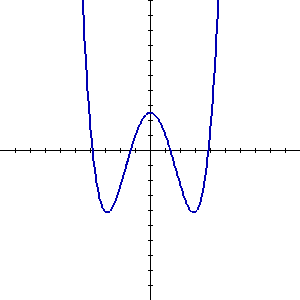
\includegraphics[width=4cm]{Differentialrechnung/achsensymm1} & 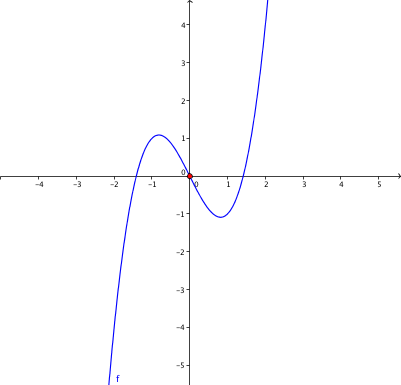
\includegraphics[width=4cm]{Differentialrechnung/Punktsym.jpg}\tabularnewline
\hline 
\end{tabular}
\end{quote}

\subsection*{Grenzwert bei Definitionslücken}
\begin{quote}
\begin{tabular}{|c|c|}
\hline 
Bsp: $f:y=\frac{x^{2}-1}{x-1}$, $D=R\setminus\left\{ 1\right\} $ & Bsp: $f:y=\frac{sin(x)}{x}$, $D=R\setminus\left\{ 0\right\} $\tabularnewline
\hline 
Kürzen möglich: $f:y=x+1$, & Kürzen nicht möglich\tabularnewline
\hline 
Definitionslücke: $x=1$ & Definitionslücke: $x=0$\tabularnewline
\hline 
Art: hebbar & Art: normale (nicht hebbare)\tabularnewline
\hline 
$lim_{x\rightarrow1}(x+1)=2$ & $lim_{x\rightarrow0}(\frac{sin(x)}{x})=1$\tabularnewline
\hline 
\end{tabular}
\end{quote}

\subsection*{Konvergenz}
\begin{quote}
Als $lim_{x\rightarrow x_{0}}f(x)=g$ - Aussage: $f(x)$ konvergiert
für $x$ gegen $x_{0}$ gegen den Grenzwert $g$ ($\ni R$).

$\forall\varepsilon\exists\delta:\forall x\mid x-x_{0}\mid<\delta,\mid f(x)-g\mid<\varepsilon$,
$g$ Grenzwert, dann konvergiert die Funktion gegen $g$
\end{quote}

\subsection*{Divergenz}
\begin{itemize}
\item Polstelle ($lim_{x\rightarrow x_{0}}=_{-}^{+}\infty$)
\item Sprung ($lim_{-\rightarrow x_{0}}\neq lim_{+\rightarrow x_{0}}$)
\item oszilliert
\end{itemize}

\subsection*{Stetigkeit}
\begin{quote}
Definition: $lim_{x\rightarrow x_{0}}f(x)=f(x_{0})$, dann ist die
Funktion stetig in $x_{0}$.\end{quote}
\begin{itemize}
\item Alle Polynome in $R$ sind stetig
\item Alle gebrochen-rationalen Funktionen in $R$ sind stetig (ausser Nullstellen
des Nenners)
\item Ist $f(x)$ in einem Intervall stetig, so ist auch $f(x)^{n}$ und
$e^{f(x)}$ im selben Intervall stetig
\end{itemize}

\section*{Grundlagen der Diff.rechnung}


\subsection*{Differenzenquotient}
\begin{verse}
\begin{tabular}{|c|}
\hline 
$Geradensteigung=m=tan(\alpha)=\frac{\Delta f}{\Delta x}=\frac{f(x_{0}+\Delta x)-f(x_{0})}{\Delta x}=\frac{y-\ddot{A}nderung}{x-\ddot{A}nderung}=\frac{y_{1}-y_{0}}{x_{1}-x_{0}}$\tabularnewline
\hline 
\end{tabular}
\end{verse}

\subsection*{Differentialquotient}
\begin{verse}
\begin{tabular}{|c|}
\hline 
$Differentialquotien=lim(Differenzenquotient)=lim_{\Delta x\rightarrow0}\frac{\Delta f(x)}{\Delta x}=lim_{\Delta x\rightarrow0}\frac{f(x_{0}+\Delta x)-f(x_{0})}{\Delta x}$\tabularnewline
\hline 
\end{tabular}
\end{verse}
Existiert de Differentialquotient so heisst die Funktion $f(x)$ an
der Stelle $x_{0}$ differenzierbar. Geometrisch bedeutet die Ableitund
der Funktion an einer Stelle deren Tangentensteigung.


\subsection*{Ableitungsfunktion}

Beispiel: Finden der abgeleiteten Funktion mit Diff.quot.:

\[
f(x)=x^{2},Diff.quot=m=\frac{f(x_{0}+\Delta x)-f(x_{0})}{\Delta x}
\]


\[
Diff.quot=\frac{(x_{0}+\Delta x)^{2}-(x_{0})^{2}}{\Delta x}=\frac{2x_{0}\Delta x+\Delta x^{2}}{\Delta x}=2x_{0}+\Delta x
\]


\[
f'(x)=lim_{\Delta x\rightarrow0}(2x_{0}+\Delta x)=2x_{0}
\]


Orte, an denen dieser Grenzwert nicht existieren kann:
\begin{itemize}
\item Graph hat eine Ecke oder Knick: $lim(links)\neq lim(rechts)$ deshalb
hat $f'(x)$ einen Sprung bei $x_{0}$.
\item Der Graph kann eine senkrechte Tangente aufweisen: $lim(f(x))=\infty$.
\end{itemize}

\subsubsection*{Tangente}
\begin{quote}
$Tangente(f(x))=f'(x)=\frac{y-y_{0}}{x-x_{0}}=m_{t}$
\end{quote}
Für Tangentengleichung:
\begin{enumerate}
\item Gleichung aufstellen: $\frac{y-y_{0}}{x-x_{0}}=f'(x_{0})$
\item $y_{0},x_{0},f'(x_{0})$ einsetzen
\item Nach y auflösen
\end{enumerate}

\subsubsection*{Normale}
\begin{quote}
$Normale(f(x))=\frac{-1}{f'(x)}=\frac{y-y_{0}}{x-x_{0}}=m_{n}$
\end{quote}
Für Normalengleichung:
\begin{enumerate}
\item Gleichung aufstellen: $\frac{y-y_{0}}{x-x_{0}}=\frac{-1}{f'(x_{0})}$
\item $y_{0},x_{0},f'(x_{0})$ einsetzen
\item Nach y auflösen
\end{enumerate}

\subsection*{Linearisierung}

Eine NICHT lineare Funktion $y=f(x)$ lässt sich in der Umgebung eines
Kurvenpunktes $P(x_{0},y_{0})$ durch die dortige Tangente ersetzen.

\[
\frac{y-y_{0}}{x-x_{0}}=f'(x)\Rightarrow y-y_{0}=f'(x_{0})(x-x_{0})\Rightarrow y=y_{0}+f'(x_{0})(x-x_{0})
\]


\[
f(x_{0}+\Delta x)\simeq y_{0}+f'(x_{0})\times\Delta x)
\]


Bsp:

\begin{tabular}{|c|c|c|cc}
\cline{1-1} \cline{3-3} 
$f(x)=x^{3}$ &  & $f'(x)=3x^{2}$ &  & \tabularnewline
\cline{1-1} \cline{3-3} 
$x_{0}=1$ & \multicolumn{1}{c}{} & \multicolumn{1}{c}{} &  & $f(1.01)\approx f(1)+f'(1)\times0.01=1.03$\tabularnewline
\cline{1-1} \cline{3-3} 
$f(1)=y_{0}=1$ &  & $f'(1)=3$ &  & $f(1.01)=(1.01)^{3}=1.030301$\tabularnewline
\cline{1-1} \cline{3-3} 
\multicolumn{1}{c}{} & \multicolumn{1}{c}{} & \multicolumn{1}{c}{} &  & Fehler: $0.3\permil$\tabularnewline
\end{tabular}


\subsection*{Ableitungsregeln}
\begin{quote}
\begin{tabular}{|c|c|c|c|c|c|c|}
\cline{1-3} \cline{5-7} 
$(c)'=c$ & $ln(x)'=\frac{1}{x}$ & $sin'=cos$ &  & $f(x)=c\cdot g(x)$ & $\implies$ & $f'(x)=c\cdot g'(x)$\tabularnewline
\cline{1-3} \cline{5-7} 
$(x^{n})'=n\cdot x^{n-1}$ & $(e^{x})'=e^{x}$ & $cos'=-sin$ &  & $f(x)=u(x)+v(x)$ & $\implies$ & $f'(x)=u'(x)+v'(x)$\tabularnewline
\cline{1-3} \cline{5-7} 
 & $(a^{x})'=a^{x}\cdot ln(a)$ & $tan'=\frac{1}{cos^{2}}$ &  & $f(x)=u(x)\cdot v(x)$ & $\implies$ & $f'(x)=u'\cdot v+u\cdot v'$\tabularnewline
\cline{2-3} \cline{5-7} 
 & $(log_{a}x)'=\frac{1}{x\cdot ln(a)}$ & $arctan'=\frac{1}{1+x^{2}}$ &  & $f(x)=\frac{u(x)}{v(x)}$ & $\implies$ & $f'(x)=\frac{u'\cdot v-u\cdot v'}{v^{2}}$\tabularnewline
\cline{3-3} \cline{5-7} 
 &  & $arcsin'=\frac{1}{\sqrt{1-x^{2}}}$ &  & $f(x)=g(h(x))$ & $\implies$ & $f'(x)=g'(h)\cdot h'(x)$\tabularnewline
\cline{3-3} \cline{5-7} 
 &  & $arccos'=\frac{-1}{\sqrt{1-x^{2}}}$ &  & $(f^{-1})'$ & $=$ & $\frac{1}{f'(x_{0})}$\tabularnewline
\end{tabular}
\end{quote}

\section*{Untersuchung von Funktionen}


\subsection*{Aussagen der 1ten Ableitung}
\begin{quote}
$f(x)$ in Intervall $I$ differenzierbar, dann:\end{quote}
\begin{itemize}
\item $f'(x)=0$ : Extremum (min/max) auf dem Intervall $I$
\item $f'(x)>0$ : $f(x)$ in $I$ monoton wachsend
\item $f'(x)<0$ : $f(x)$ in $I$ monoton fallend\end{itemize}
\begin{quote}
Das heisst, dass das Vorzeichen der ersten Ableitung uns sagt, ob
die Funktion steigt oder fällt.
\end{quote}

\subsection*{Aussagen der 2ten Ableitung}
\begin{quote}
$f(x)$ in Intervall $I$ 2 mal differenzierbar, dann:\end{quote}
\begin{itemize}
\item \textbf{$f''(x)>0$} : $f'(x)$ ist (streng) monoton wachsend : $f(x)$
ist \textbf{konvex}
\item \textbf{$f''(x)<0$ }: $f'(x)$ ist (streng) monoton fallend : $f(x)$
ist \textbf{konkav}
\end{itemize}

\subsection*{Extremwerte}
\begin{quote}
Durch die erste Ableitung $f'(x)=0$ erhalten wir Kandidatstellen
$x_{i}$ für Minimum und Maximum.\end{quote}
\begin{itemize}
\item Ist in der Umgebung der Stelle $x_{i}$ die Funktion $f(x)$ \textbf{konkav},
so liegt ein \textbf{Maximum} vor.
\item Ist in der Umgebung der Stelle $x_{i}$ die Funktion $f(x)$ \textbf{konvex},
so liegt ein \textbf{Minimum} vor.
\end{itemize}

\subsection*{Wendepunkte}
\begin{quote}
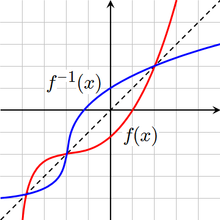
\includegraphics[width=4cm]{Differentialrechnung/220px-Inverse_Function_Graph}$f(x)$
ist im Intervall $I$ 3 mal differenzierbar, dann:\end{quote}
\begin{itemize}
\item $f''=0,f'''<0$ : blau : Links- zu Rechtskurve
\item $f''=0,f'''>0$ : rot : Rechts- zu Linkskurve
\end{itemize}

\section*{Newtonverfahren}
\begin{quote}
Newtonsches Tangentenverfahren:
\[
x_{n}=x_{n-1}-\frac{f(x_{n-1})}{f'(x_{n-1})},n=1,2,3,...
\]


Kriterium, das für Startwert und während des ganzen Verfahrens gelten
soll:
\[
\mid\frac{f\cdot\text{f'}}{(f'')^{2}}\mid<1
\]


Startwert: nicht Stellen, an denen die Kurventangente (fast) parallel
zur x-Achse verläuft.
\end{quote}

\section*{Bernoulli de l'Hopital}


\subsection*{Mittelwertsatz der Diff.rechnung}

\begin{tabular}{|c|c|}
\hline 
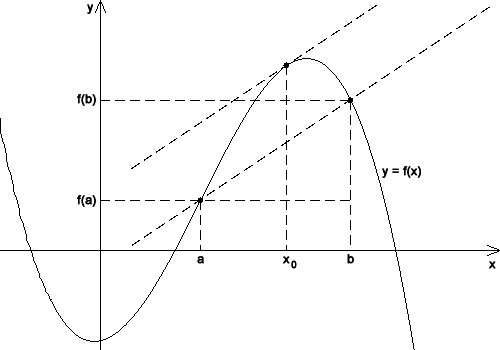
\includegraphics[width=5cm]{Differentialrechnung/MittelwertsatzD} & \includegraphics[width=5cm]{Differentialrechnung/550px-Satz_von_Rolle\lyxdot svg}\tabularnewline
\hline 
\hline 
$f(x)$ in $[a,b]$ stetig und differenzierbar in $]a,b[$ , dann
$\exists\xi\in]a,b[$ : & Spezialfall: Satz von Rolle \tabularnewline
\hline 
$\frac{f(b)-f(a)}{b-a}=f'(\xi)$ & $f(a)=f(b)$\tabularnewline
\hline 
\end{tabular}


\subsection*{Allgemeiner Mittelwertsatz der Diff.rechnung}
\begin{quote}
$f(x),g(x)$ in $[a,b]$ stetig und in$]a,b[$ differenzierbar sowie
$g'(x)\neq0$ in $]a,b[$, dann $\exists\xi\in]a,b[$:

\[
\frac{f(b)-f(a)}{g(b)-g(a)}=\frac{f'(\xi)}{g'(\xi)}
\]

\end{quote}

\subsection*{Regel von Bernoulli de l'Hopital}
\begin{quote}
Die Funktionen seien auf einen offenen Intervall stetig: $]a,b[$
(wobei das Intervall auch unendlich sein kann).

Falls:
\[
lim_{x\rightarrow b}f(x)=lim_{x\rightarrow b}g(x)=0\: oder\: lim_{x\rightarrow b}f(x)=lim_{x\rightarrow b}g(x)=_{-}^{+}\infty\: und\: lim_{x\rightarrow b}\frac{f'}{g'}=d
\]


so ist: 
\[
lim_{x\rightarrow b}\frac{f(x)}{g(x)}=lim_{x\rightarrow b}\frac{f'(x)}{g'(x)}=d
\]
\end{quote}




\part*{Potenzen}


\section*{Gesetze}

\begin{tabular}{|c|c|c|c|c|}
\hline 
$a^{n}\cdot a^{m}=a^{n+m}$ & $a^{n}:a^{m}=a^{n-m}$ & $a^{n}\cdot b^{n}=(a\cdot b)^{n}$ & $\frac{a^{n}}{b^{n}}=(\frac{a}{b})^{n}$ & $(a^{n})^{m}=a^{n\cdot m}$\tabularnewline
\hline 
$a^{-n}=\frac{1}{a^{n}}$ & $\sqrt[n]{a}=a^{\frac{1}{n}}$ & $\sqrt[n]{a^{m}}=(\sqrt[n]{a})^{m}=a^{\frac{m}{n}}$ & $-a^{n}=-(a^{n})$ & $(-a)^{n}=(-1)^{n}\cdot a^{n}$\tabularnewline
\hline 
\end{tabular}


\part*{Additionstheoreme}


\section*{Sätze}
\begin{itemize}
\item $sin(\alpha+\beta)=sin(\alpha)\cdot cos(\beta)+cos(\alpha)\cdot sin(\beta)$
\item $sin(\alpha-\beta)=sin(\alpha)\cdot cos(\beta)-cos(\alpha)\cdot sin(\beta)$
\item $cos(\alpha+\beta)=cos(\alpha)\cdot cos(\beta)+sin(\alpha)\cdot sin(\beta)$
\item $sin(\alpha-\beta)=cos(\alpha)\cdot cos(\beta)-sin(\alpha)\cdot sin(\beta)$
\end{itemize}

\part*{Trigonometrische Funktionen}


\section*{Definition}
\begin{verse}
\begin{tabular}{ll}
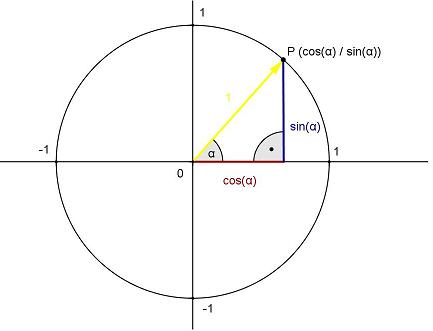
\includegraphics[height=6cm]{Repetition/Einheitskreis} & 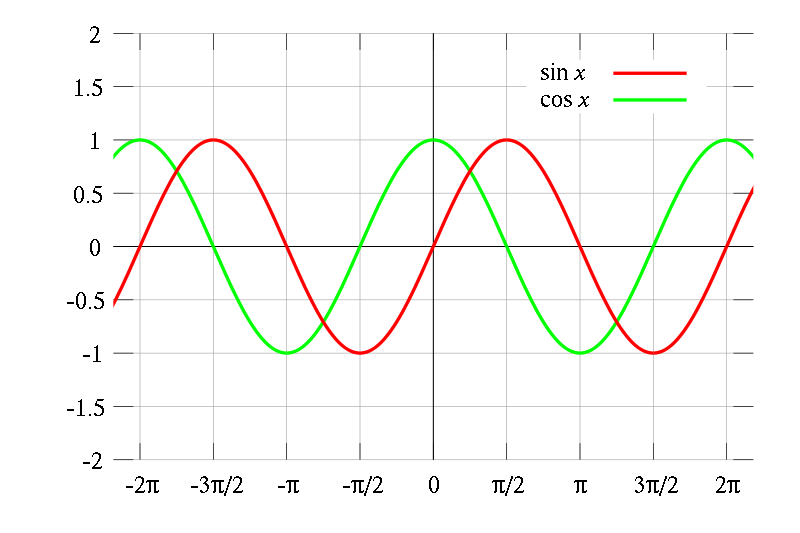
\includegraphics[height=6cm]{Repetition/Sin_Cos}\tabularnewline
\end{tabular}
\end{verse}
\begin{tabular}{|c|c|c|}
\hline 
$sin(x)=cos(x)\cdot tan(x)$ & $cos(x)=\frac{sin(x)}{tan(x)}$ & $tan(x)=\frac{sin(x)}{cos(x)}$\tabularnewline
\hline 
\end{tabular}


\section*{Bogenmass eines Winkels}

Länge des zugehörigen Bogens im Einheitskreis.
\begin{verse}
$\alpha=90\text{°}\leftrightarrow\alpha=\frac{\Pi}{2}$

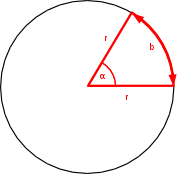
\includegraphics[height=3cm]{Repetition/Bogenmass}
\end{verse}

\section*{Anwendung in der Schwingungslehre}
\begin{verse}
\begin{tabular}{lll}
A = Amplitude & w = Kreisfrequenz & $\varphi$ = Phase der Schwingung\tabularnewline
 &  & Periode p = $\frac{alte\, Periode}{w}$, also bei sin/cos z.B.: $\frac{2\Pi}{w}$\tabularnewline
\end{tabular}

\begin{tabular}{|c|}
\hline 
$y=A\cdot sin[w\cdot t+\varphi]=A\cdot sin[\, w\cdot(t+\frac{\varphi}{w})\,]$\tabularnewline
\hline 
\end{tabular}
\end{verse}
Allgemein:
\begin{enumerate}
\item Streckung in y-Richtung mit Faktor a $\Rightarrow$ Wertebereich {[}-a,a{]}
\item Streckung in x-Richtung mit Faktor $\frac{1}{b}\Rightarrow$neue Periode
$\frac{alte\, Periode}{b}$, also bei sin/cos z.B.: $\frac{2\Pi}{b}$
\item Verschiebung in x-Richtung um $-\frac{\varphi}{b}$\end{enumerate}
\begin{verse}
\begin{tabular}{|c|}
\hline 
$y=a\cdot f[\, b\cdot(x-c)\,]+d$\tabularnewline
\hline 
\end{tabular}
\end{verse}
Beispiel:
\begin{verse}
\begin{tabular}{|c|}
\hline 
$y=3\cdot sin[\frac{1}{2}\cdot x+\frac{\Pi}{4}]=3\cdot sin[\,\frac{1}{2}\cdot(x+\frac{\Pi}{2})\,]$\tabularnewline
\hline 
\end{tabular}

\begin{tabular}{cccc}
Amplitude = 3 & Kreisfrequenz = $\frac{1}{2}$ & $\Rightarrow$Neue Periode = $\frac{2\Pi}{w}=\frac{2\Pi}{\frac{1}{2}}=4\Pi$ & Verschiebung in x-Richtung = $-\frac{\Pi}{2}$\tabularnewline
\end{tabular}

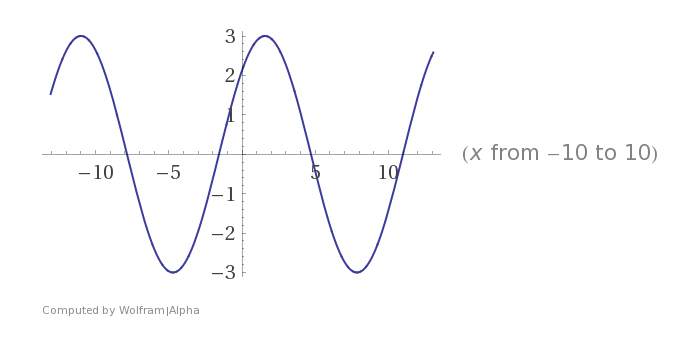
\includegraphics[height=5cm]{Repetition/Schwingung}
\end{verse}

\part*{Exponetial- und Logarithmusfunktion}

Jede Exponentielle Funktion lässt sich mit der Basis e schreiben:

\begin{tabular}{|c|}
\hline 
$y=b^{x}=(e^{ln(b)})^{x}$\tabularnewline
\hline 
\end{tabular}


\section*{Wachstums- und Zerfallfunktion}

Allgemein:

\begin{tabular}{ll}
$a=$Wert für $t^{0}$, ``Startwert'' & $b=$Wachstumsfaktor pro Zeiteinheit\tabularnewline
$t=$Zeiteinheit & $\Delta t=$Zeitdifferenz z.B. $t^{2}-t^{1}$\tabularnewline
\end{tabular}
\begin{verse}
\begin{tabular}{|c|}
\hline 
$y=a\cdot b^{t}$\tabularnewline
\hline 
\end{tabular}

\begin{tabular}{cc}
\textbf{Wachstumsfunktion: b > 1,} & \textbf{Zerfallsfunktion: 0 < b < 1 }\tabularnewline
\end{tabular}
\end{verse}
Umformungen:
\begin{verse}
\begin{tabular}{|c|}
\hline 
$b^{\Delta t}=\frac{f(t_{2})}{f(t_{1})}\Rightarrow b=\sqrt[\Delta t]{\frac{f(t_{2})}{f(t_{1})}}$\tabularnewline
\hline 
\end{tabular}
\end{verse}
Halbwertszeit:
\begin{verse}
\begin{tabular}{|c|}
\hline 
$b^{\Delta t}=\frac{1}{2}\Rightarrow\Delta t\cdot ln(b)=ln(\frac{1}{2})\Rightarrow\Delta t=\frac{ln(\frac{1}{2})}{ln(b)}$\tabularnewline
\hline 
\end{tabular}
\end{verse}
Verdoppelungszeit:
\begin{verse}
\begin{tabular}{|c|}
\hline 
$b^{\Delta t}=2\Rightarrow\Delta t\cdot ln(b)=ln(2)\Rightarrow\Delta t=\frac{ln(2)}{ln(b)}$\tabularnewline
\hline 
\end{tabular}
\end{verse}

\section*{Logarithmusfunktion}

Rechenregeln:
\begin{verse}
\begin{tabular}{|c|}
\hline 
$log_{a}(u\cdot v)=log_{a}(u)+log_{a}(v)$\tabularnewline
\hline 
$log_{a}(\frac{u}{v})=log_{a}(u)-log_{a}(v)$\tabularnewline
\hline 
$log_{a}(u^{k})=k\cdot log_{a}(u)$\tabularnewline
\hline 
$log_{a}(\sqrt[n]{u})=\frac{1}{n}\cdot log_{a}(u)$\tabularnewline
\hline 
\end{tabular}
\end{verse}
Allgemein:
\begin{verse}
\begin{tabular}{|c|}
\hline 
$y=a^{x}\Rightarrow ln(y)=x\cdot ln(a)\Rightarrow x=\frac{ln(y)}{ln(a)}$\tabularnewline
\hline 
\end{tabular}

\begin{tabular}{|c|}
\hline 
$y=a^{x}\Rightarrow log_{a}(y)=x\cdot log_{a}(a)\Rightarrow x=log_{a}(y)$ \tabularnewline
\hline 
\end{tabular}
\end{verse}
Umkehrfunktion:
\begin{verse}
\begin{tabular}{|c|}
\hline 
$y=log_{a}(x)$\tabularnewline
\hline 
\end{tabular}
\end{verse}
Basiswechsel:
\begin{verse}
\begin{tabular}{|c|}
\hline 
$log_{a}(x)=\frac{log_{10}(x)}{log_{10}(a)}=\frac{ln(x)}{ln(a)}$\tabularnewline
\hline 
\end{tabular}
\end{verse}
Umformungsbeispiele:
\begin{verse}
\begin{tabular}{|l|l|l|}
\hline 
$log_{10}(x)=-4.0404$ & $\Rightarrow$ & $x=10^{-4.0404}=\frac{1}{10^{4.0404}}$\tabularnewline
\hline 
$ln(x)=-9.0907$ & $\Rightarrow$ & $x=e^{-9.0907}=\frac{1}{e^{9.0907}}$\tabularnewline
\hline 
$log_{3}(x)=5$ & $\Rightarrow$ & $x=3^{5}=243$\tabularnewline
\hline 
\end{tabular}\end{verse}

\end{lyxcode}

\end{document}
